\normaltrue
\correctionfalse

%\UPSTIidClasse{11} % 11 sup, 12 spé
%\newcommand{\UPSTIidClasse}{12}

\exer{Roue motrice de chariot élévateur  $\star$ \label{A5:05:74}}
\setcounter{numques}{0}
\UPSTIcompetence[2]{A5-05}
\UPSTIcompetence[2]{A5-04}

\index{Compétence A5-05}
\index{Compétence A5-04}

\index{GPS}
\index{Spécification géométrique des produits}
\index{Roue motrice}

\ifcorrection
\else
\textbf{Pas de corrigé pour cet exercice.}
\fi

\ifprof
\else


On considère le caisson d'un train aterrissage avant d'un avion. 

\begin{minipage}[c]{.5\linewidth}
\begin{center}
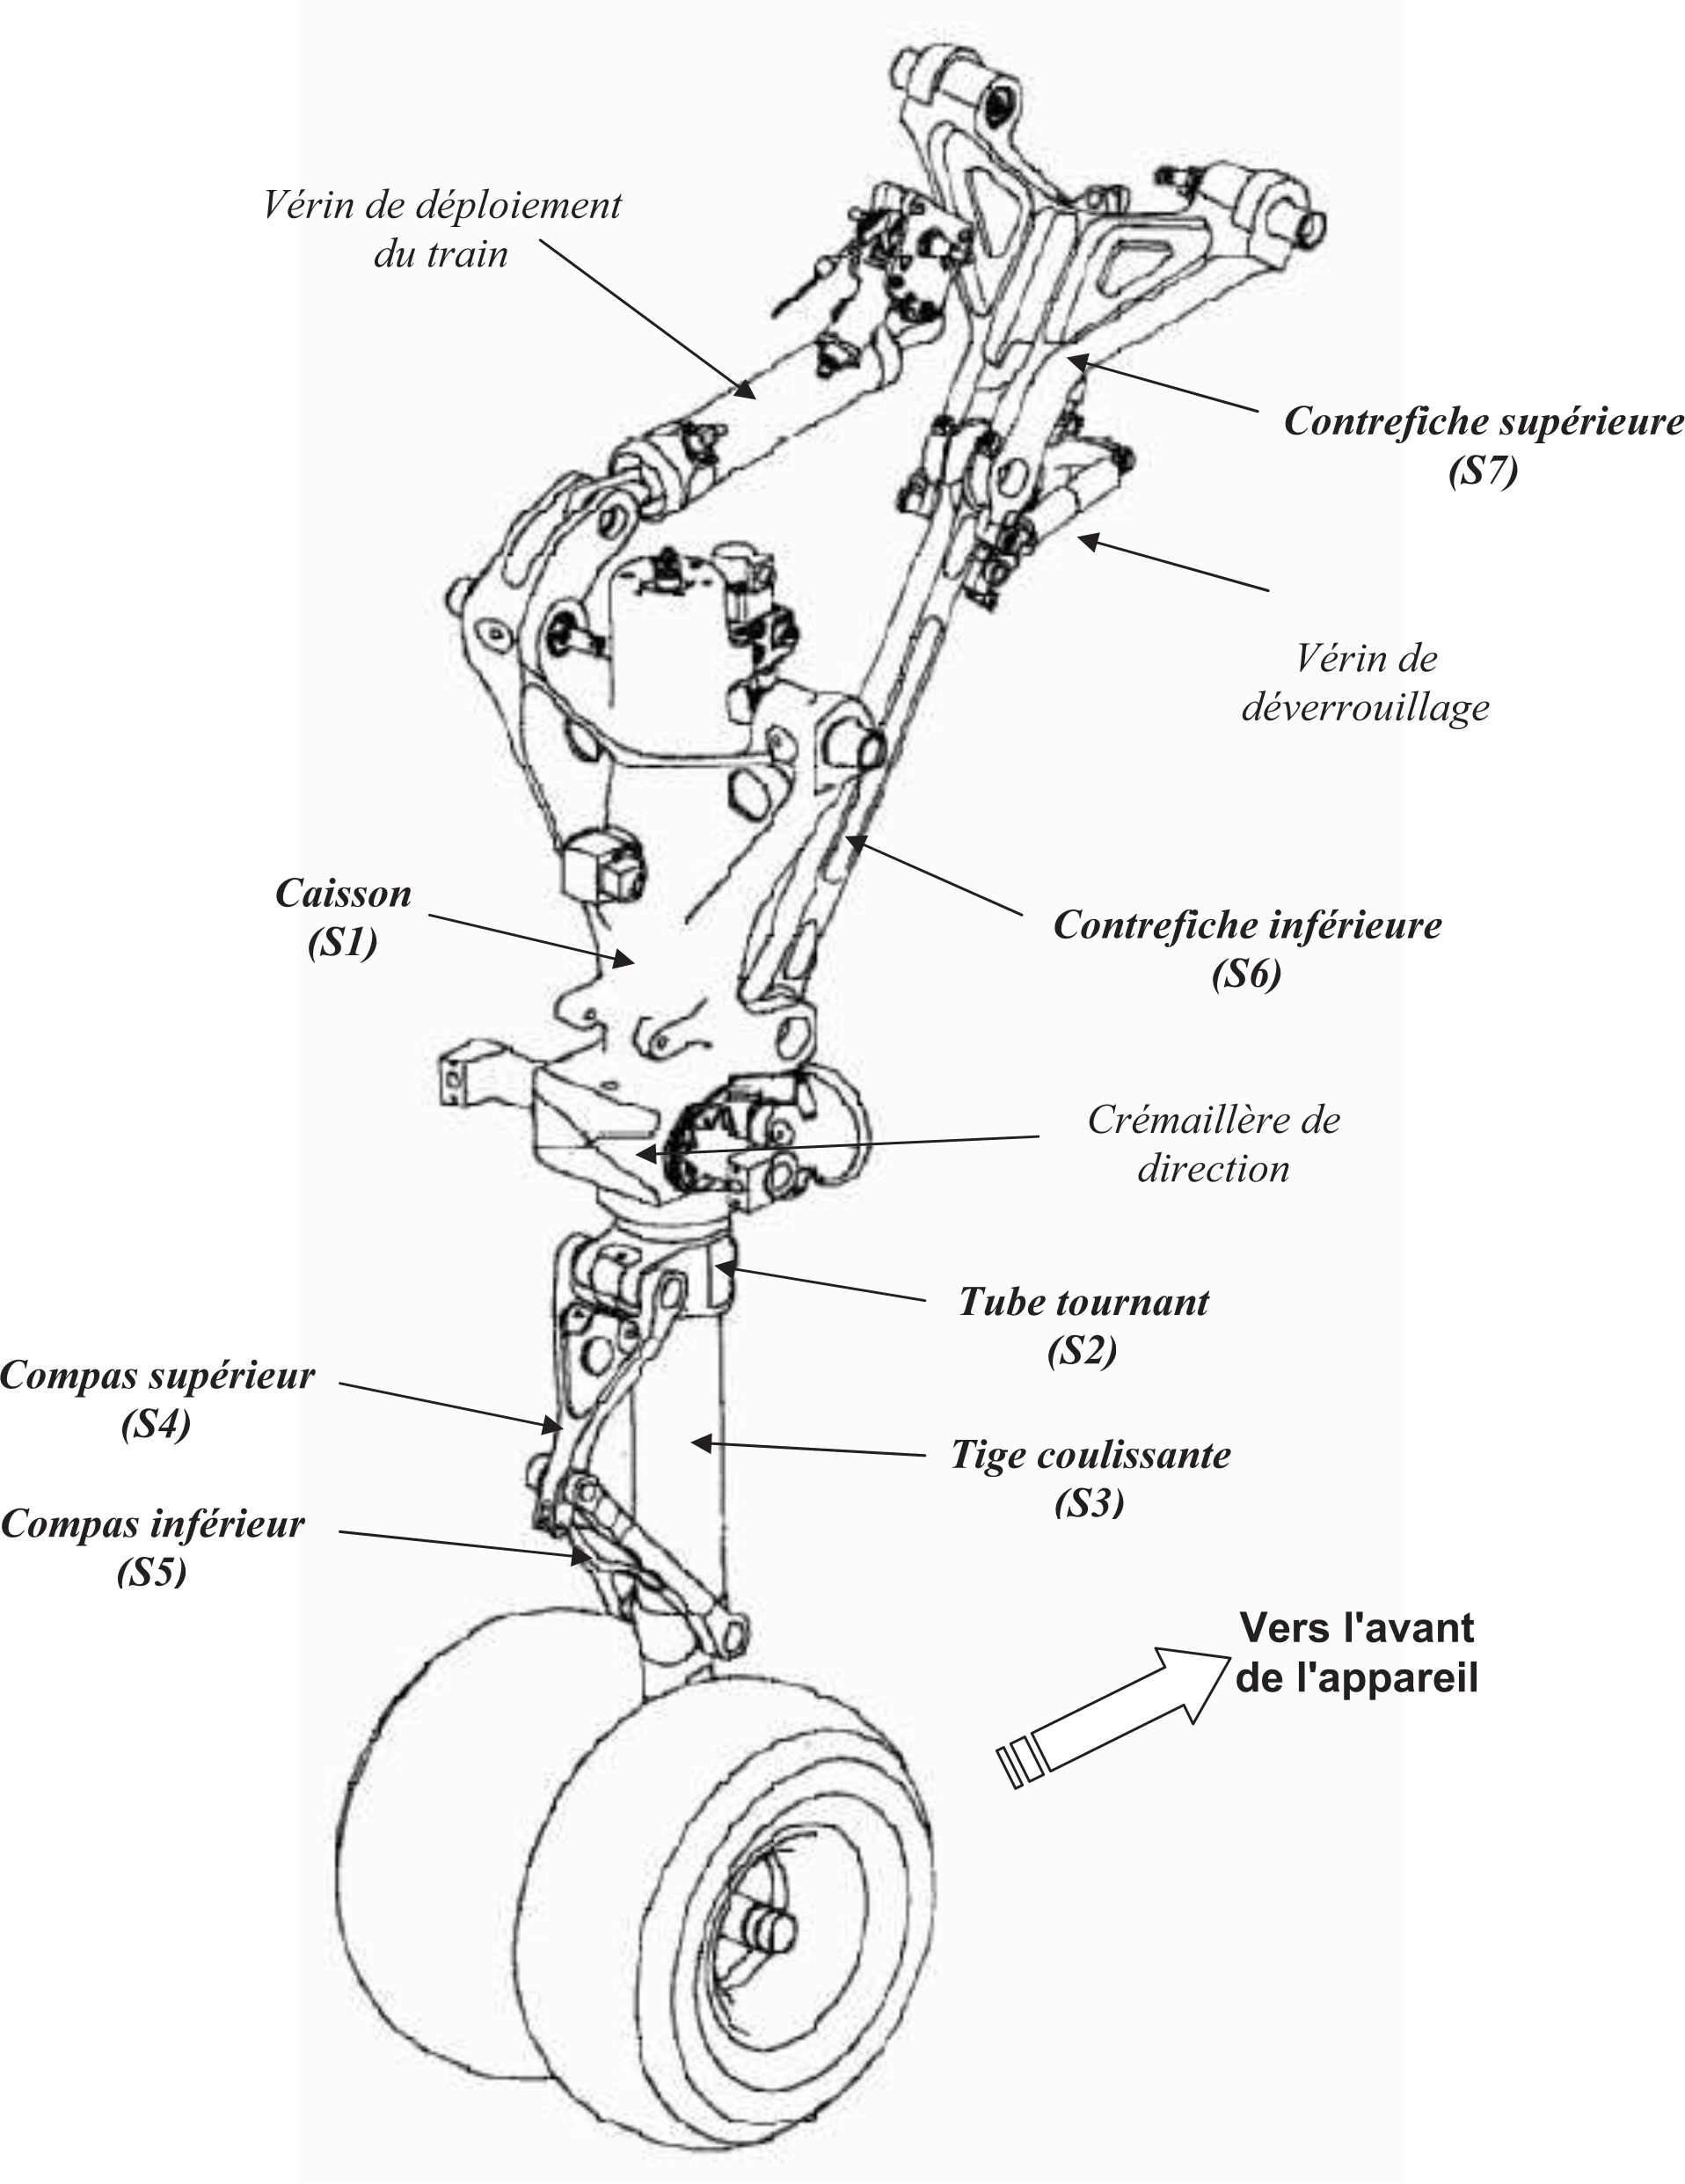
\includegraphics[width=.7\linewidth]{75_01}
\end{center}
\end{minipage} \hfill
\begin{minipage}[c]{.5\linewidth}
\begin{center}
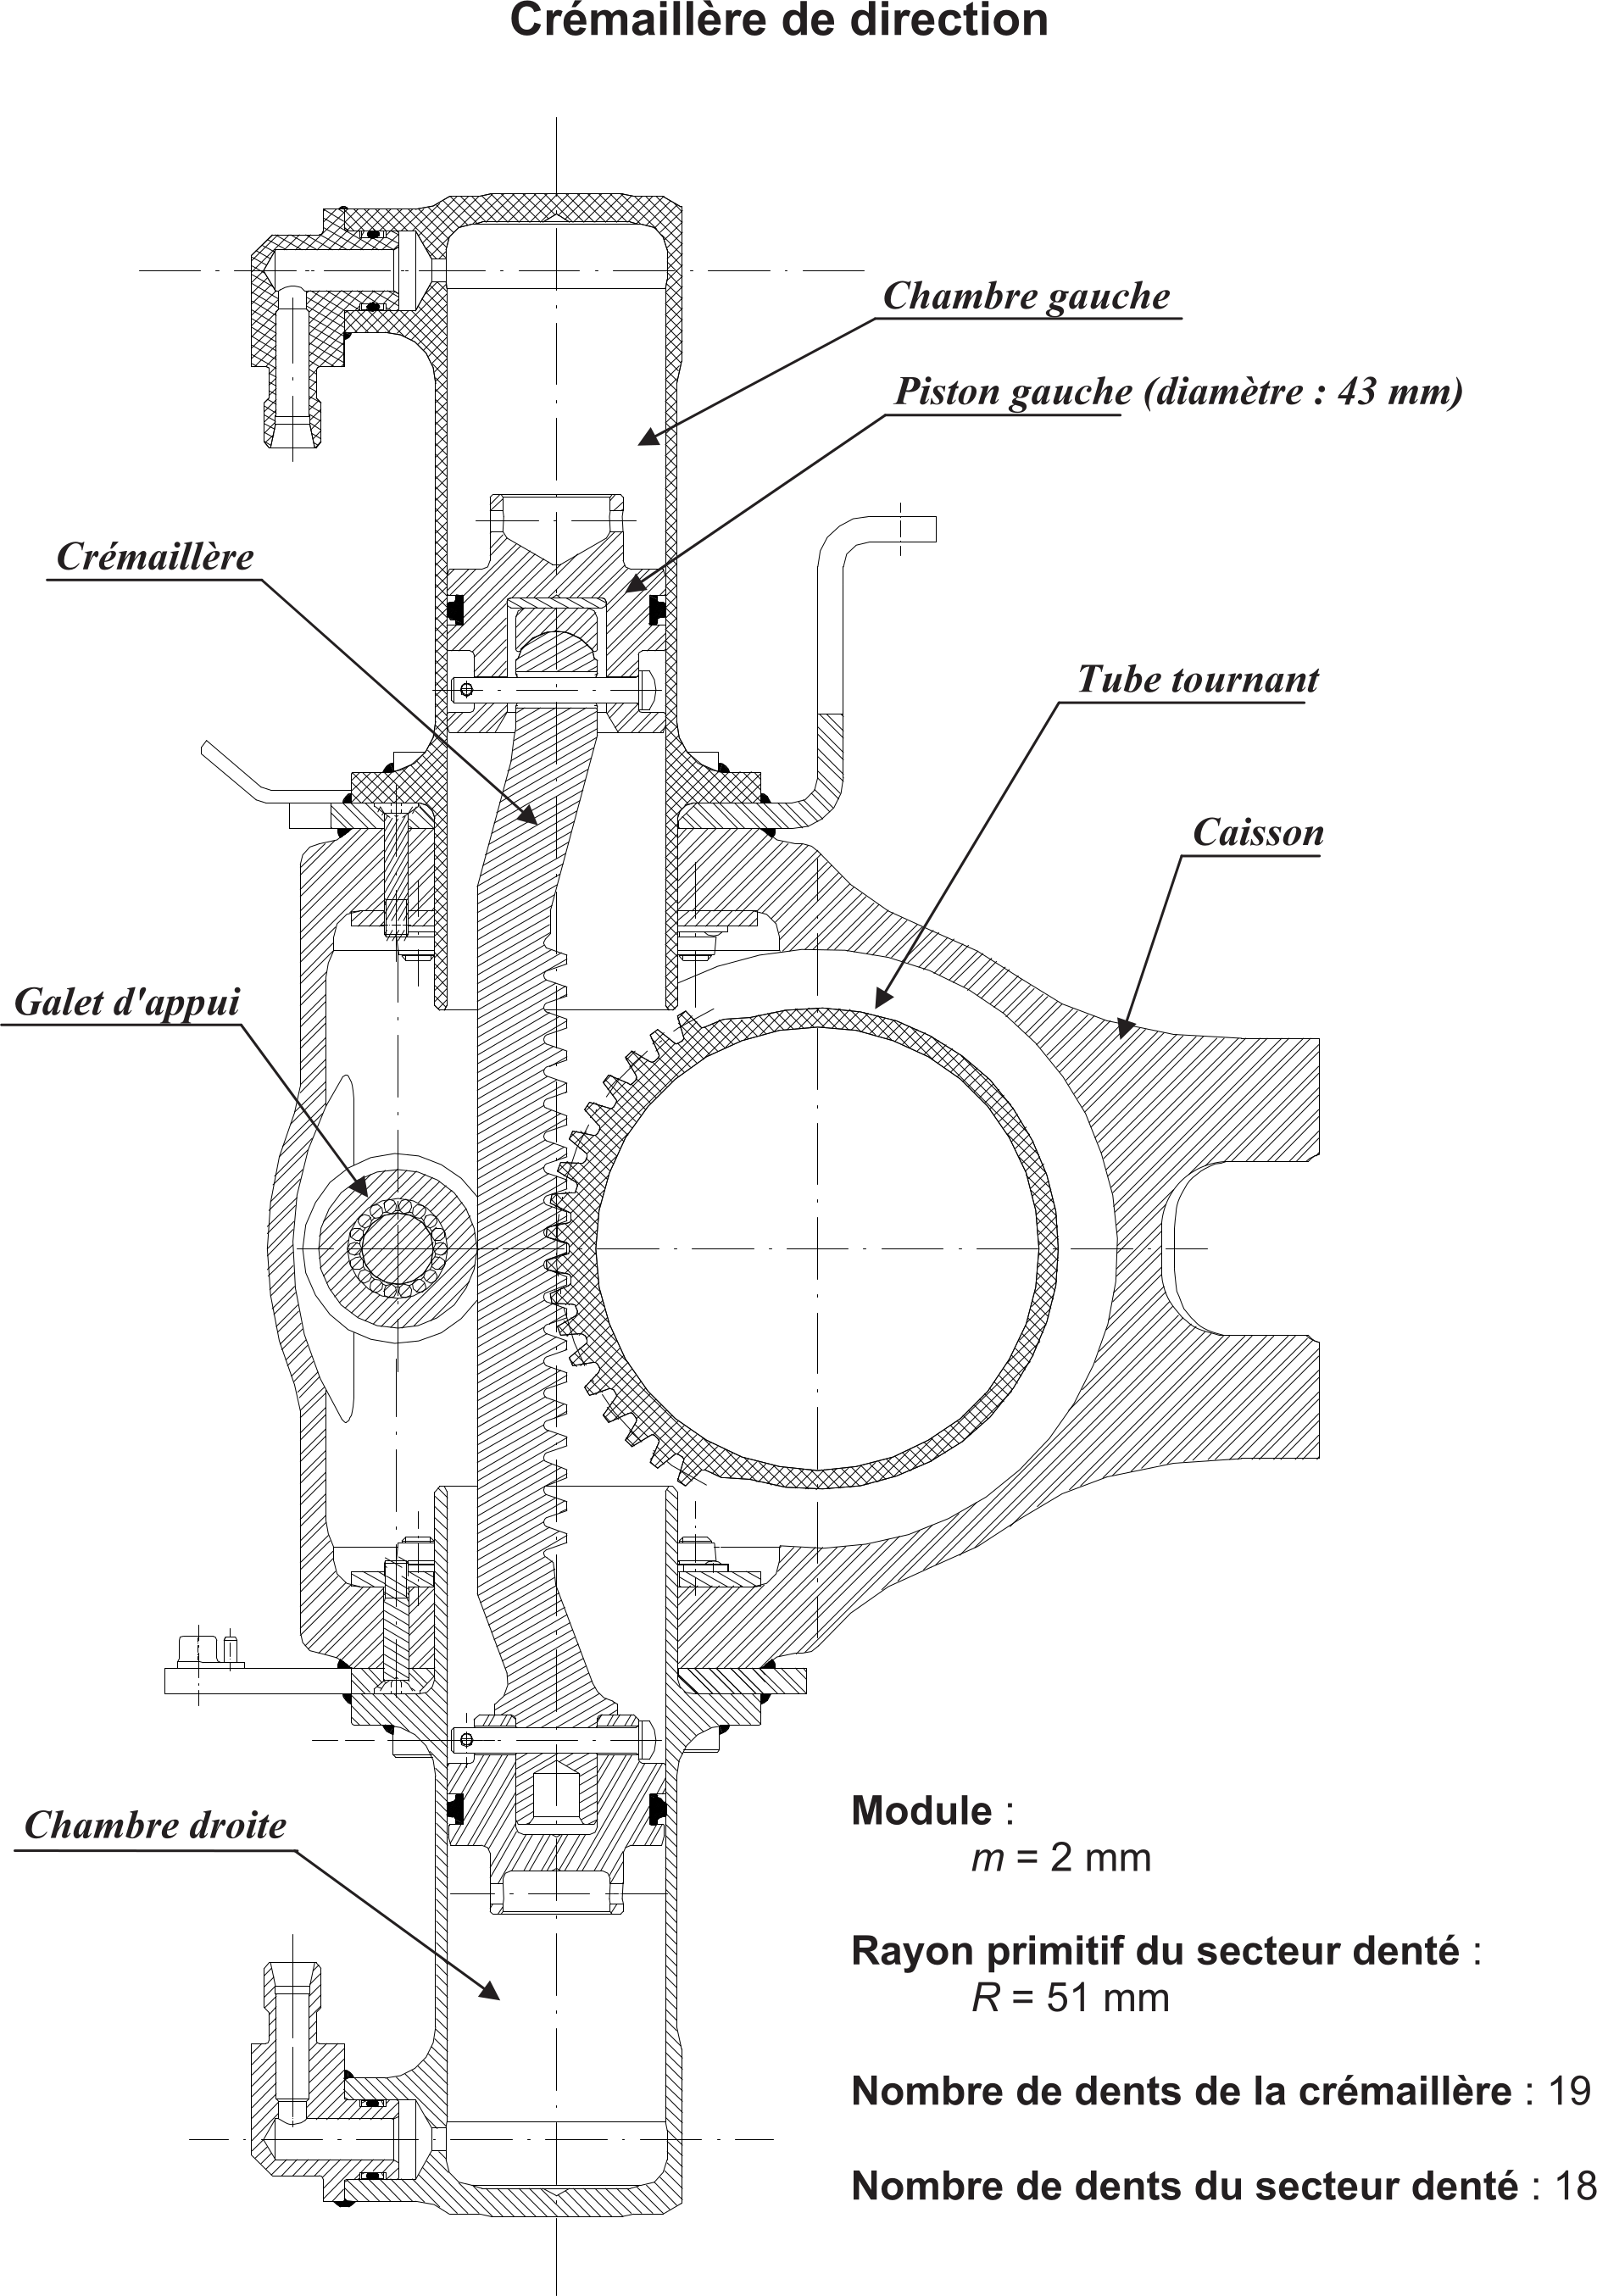
\includegraphics[width=.7\linewidth]{75_02}
\end{center}
\end{minipage} \hfill


\fi



\question{Justifier pourquoi les surfaces J et H ont été choisies comme éléments de référence ?}
\ifprof
\else
\fi

\question{Justifier pourquoi les surfaces S et T ont été choisies comme éléments de référence ?}
\ifprof
\else
\fi

\question{Décoder les spécifications suivantes : 
\includegraphics[height=0.8cm]{75_04}.
 Dans cette spécification l'enveloppe est implicite. Que cela signifie-t-il ? Tracer le gabarit associé. $\phi 42,5 H7 =32,5 ^{\begin{pmatrix}+25 \\ +0\end{pmatrix}}$}
\ifprof
\else
\fi

\question{Décoder la spécification suivante 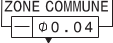
\includegraphics[height=0.8cm]{75_06}.}
\ifprof
\else
\fi

\question{Décoder la spécification suivante 
\includegraphics[height=0.8cm]{75_07}.}
\ifprof
\else
\fi

\question{Décoder la spécification suivante 
\includegraphics[height=1.2cm]{75_08}.}
\ifprof
\else
\fi

\question{Décoder la spécification suivante 
\includegraphics[height=0.8cm]{75_09}.}
\ifprof
\else
\fi



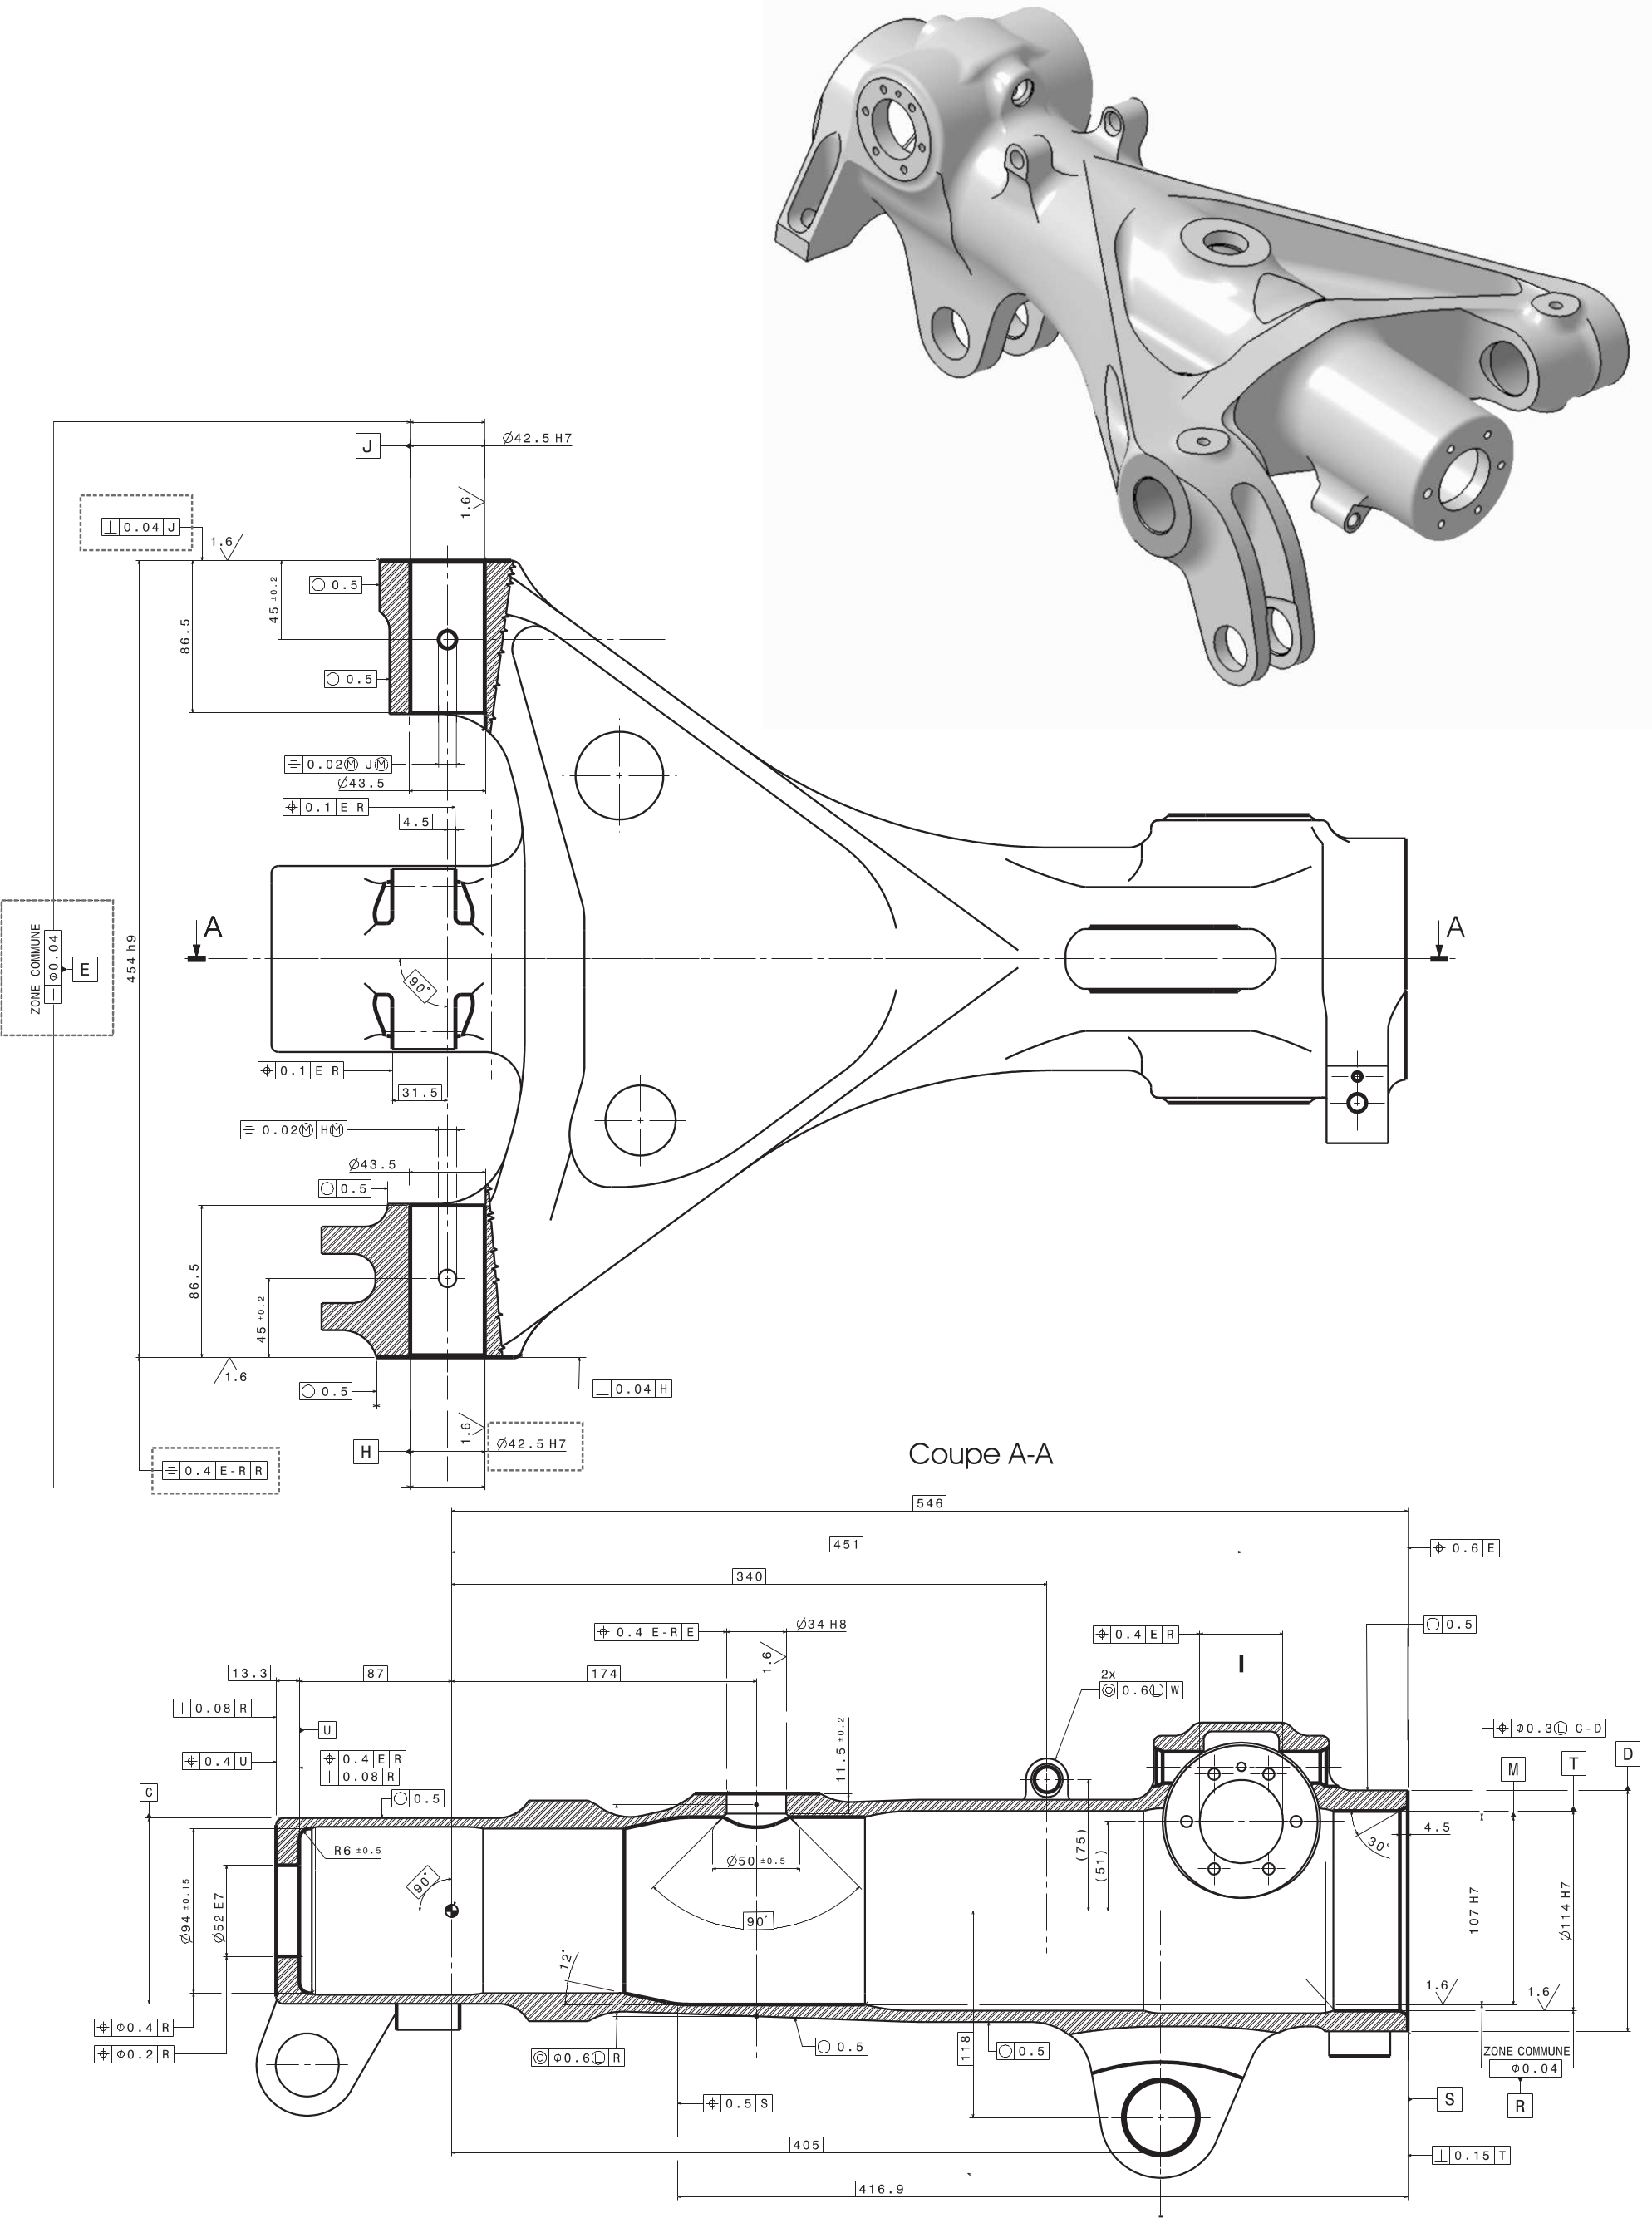
\includegraphics[width=\linewidth]{75_03.png}

\ifprof
\else
\begin{flushright}
\footnotesize{Corrigé  voir \ref{A5:05:75}.}
\end{flushright}%
\fi 